%%%%%%%%%%%%%%%%%%%%%%%%%%%%%%%%%%%%%%%%%
% A0 portrait poster for:
% A Language Model from 1913: Pretraining on Historical Text
%
% The visual settings intentionally follow poster/poster-example/poster.tex.
%%%%%%%%%%%%%%%%%%%%%%%%%%%%%%%%%%%%%%%%%

\PassOptionsToPackage{table}{xcolor}
\documentclass[portrait,a0paper,fontscale=0.42]{baposter}

\usepackage{graphicx}
\graphicspath{{figures/}}
\usepackage{amsmath}
\usepackage{amssymb}
\usepackage{array}
\usepackage{booktabs}
\usepackage[shortlabels]{enumitem}
\usepackage{makecell}
\usepackage{multirow}
\usepackage{multicol}
\usepackage{palatino}
\usepackage[font=small,labelfont=bf]{caption}
\usepackage{xcolor}
\usepackage{xspace}
\usepackage{tikz}
\usetikzlibrary{arrows.meta,positioning,shapes.geometric}

\setlist[itemize]{leftmargin=*,itemsep=1pt,topsep=2pt}
\setlength{\columnsep}{1.5em}
\setlength{\columnseprule}{0mm}

\definecolor{lightblue}{rgb}{0.145,0.6666,1}
\definecolor{tticblue}{RGB}{0,94,184}
\definecolor{PKUred}{HTML}{94070A}
\definecolor{DarkBlue}{HTML}{00274C}
\definecolor{Maize}{HTML}{FFCB05}
\definecolor{Highlight}{HTML}{DC7B22}
\definecolor{SoftBlue}{HTML}{EBF3FE}
\definecolor{SoftGray}{HTML}{F4F4F5}
\definecolor{DeepGreen}{HTML}{256D4A}

\newcommand{\twlm}{\textsc{TypewriterLM}\xspace}
\newcommand{\twcorpus}{\textsc{TypewriterCorpus}\xspace}
\newcommand{\histevent}{\textsc{History-Event}\xspace}
\newcommand{\histlima}{\textsc{History-LIMA}\xspace}
\newcommand{\histself}{\textsc{History-SelfInstruct}\xspace}
\begin{document}

\large
\begin{poster}
    {
        headerborder=open,
        colspacing=0.5em,
        bgColorOne=white,
        bgColorTwo=white,
        background=plain,
        borderColor=white,
        headerColorOne=DarkBlue,
        headerColorTwo=DarkBlue,
        headershade=plain,
        headerFontColor=white,
        boxColorOne=white,
        textborder=roundedsmall,
        eyecatcher=true,
        headerheight=0.1\textheight,
        headershape=roundedright,
        headerfont=\Large\bf\textsc,
        linewidth=2pt,
        columns=6
    }
    {}
    {
        \fontsize{20}{21}\selectfont
        \begin{minipage}{0.95\textwidth}
            \centering
            \textbf{\textcolor{DarkBlue}{A Language Model from 1913: Pretraining on Historical Text}}
        \end{minipage}
    }
    {
        \fontsize{12.4}{13.2}\selectfont
        \vspace{3pt}
        Xiaoxi Luo\textsuperscript{1,2},
        Zachary Shinnick\textsuperscript{3,4},
        Niclas Griesshaber\textsuperscript{4,5},
        Yixuan Wang\textsuperscript{1,2},
        Junchi Yu\textsuperscript{4},
        Freda Shi\textsuperscript{1,2},
        Philip Torr\textsuperscript{4},
        Yao Lu\textsuperscript{6}\\[3pt]
        \fontsize{8.8}{9.4}\selectfont
        \textsuperscript{1}University of Waterloo \quad
        \textsuperscript{2}Vector Institute \quad
        \textsuperscript{3}Adelaide University\\
        \textsuperscript{4}University of Oxford \quad
        \textsuperscript{5}Oxford Centre for Economic and Social History\\
        \textsuperscript{6}University College London
    }
    {
        \begin{minipage}{180pt}
            \centering
            \vspace{-12pt}
            
\includegraphics[height=34pt]{uw.png}
            \hspace{10pt}
            
\includegraphics[height=34pt]{vector.png}\\[5pt]
            
\includegraphics[width=145pt]{conference.png}
        \end{minipage}
    }

    \headerbox{}{name=teaser,column=0,span=3,row=0,textborder=none,boxshade=none,
        headerborder=none,boxheaderheight=0pt,boxpadding=0pt}{
        \centering
        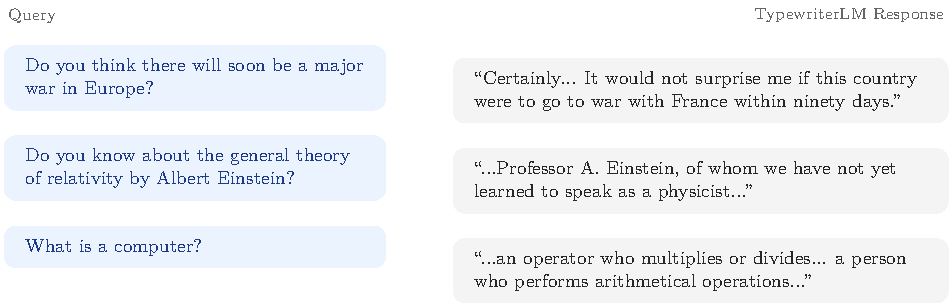
\includegraphics[width=0.98\linewidth]{teaser.pdf}\\[-2pt]
        \small\textbf{Teaser.} Probing \twlm on ``future'' events.
    }

    \headerbox{Takeaways}{name=takeaways,column=3,span=3,aligned=teaser,bottomaligned=teaser,
        borderColor=PKUred,headerColorOne=PKUred,headerColorTwo=DarkBlue}{
        \begin{itemize}
            \item \textbf{54B historical tokens} produce a capable 7.24B model with a \textbf{1913 cutoff}.
            \item \textbf{Leakage-aware post-training} constrains every assistant response to pre-1913 source language.
            \item \textbf{The cutoff is visible:} History LMs become more surprised by post-cutoff events.
            \item \textbf{Capability remains non-trivial:} \twlm is competitive with existing History LMs on historically aligned benchmarks.
            \item \textbf{Metadata leakage is small but real} and requires document-level filtering.
        \end{itemize}

        \vspace{4pt}
        \colorbox{SoftBlue}{\parbox{0.93\linewidth}{\centering
            \textbf{History LMs must be evaluated for capability and cutoff adherence together.}}}
    }

    \headerbox{1. Pretraining}{name=pretrain,column=0,span=3,below=teaser,borderColor=DarkBlue}{
        \centering
        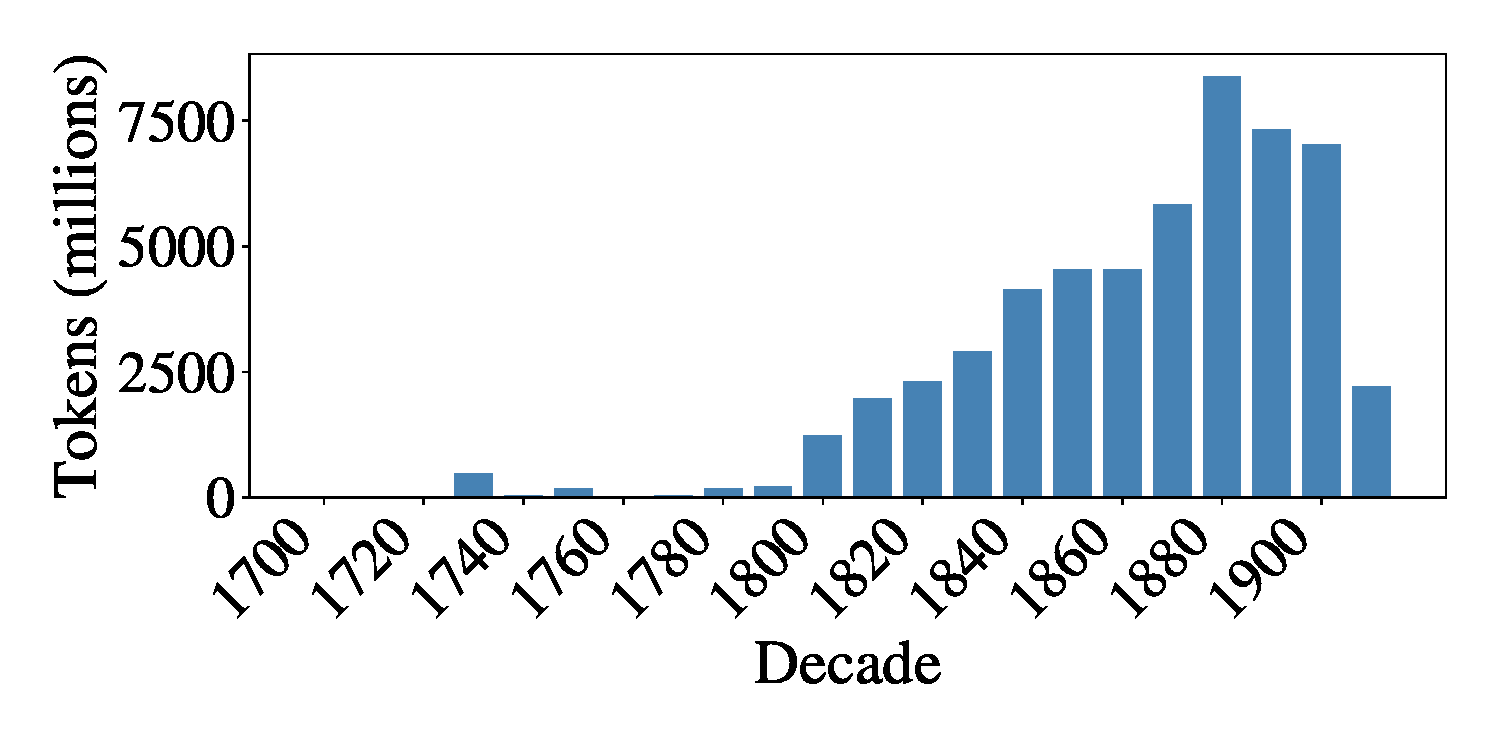
\includegraphics[width=0.88\textwidth]{token_count_by_year.pdf}\\[-3pt]
        \small\textbf{Figure 1.} \twcorpus tokens by decade.

        \vspace{5pt}
        \colorbox{SoftBlue}{\parbox{0.88\textwidth}{\centering
            \textbf{54B corpus tokens} \quad \textbf{140B training tokens} \quad \textbf{2.59 epochs}}}

        \vspace{7pt}
        \begin{minipage}[t]{0.42\textwidth}
            \small
            \textcolor{DarkBlue}{\textbf{Model}}
            \begin{itemize}
                \item Llama 3-style decoder, 32 layers
                \item 7.24B parameters; 8,192 context
                \item 32K custom historical BPE
                \item GQA: 32 query / 8 KV heads
            \end{itemize}
            \textcolor{DarkBlue}{\textbf{Leakage-aware cleaning}}
            \begin{itemize}
                \item OCR-quality and fragment filters
                \item Repair split words and OCR artifacts
                \item Remove provenance, URLs, HTML, and editorial metadata
            \end{itemize}
        \end{minipage}
        \hfill
        \begin{minipage}[t]{0.54\textwidth}
            \centering
            \scriptsize
            \resizebox{\linewidth}{!}{%
                \begin{tabular}{llrr}
                    \toprule
                    \textbf{Dataset} & \textbf{Domain} & \textbf{Tok. (M)} & \textbf{\%} \\
                    \midrule
                    Institutional & Books & 52,736 & 97.68 \\
                    BL Books & Books & 915 & 1.69 \\
                    Hansard & Parliamentary & 193 & 0.36 \\
                    Royal Society & Scientific & 70 & 0.13 \\
                    Old Bailey & Court & 39 & 0.07 \\
                    CLMET & Literary & 31 & 0.06 \\
                    CED & Dialogues & 0.67 & $<$0.01 \\
                    Lampeter & Tracts & 0.35 & $<$0.01 \\
                    CLME Prose & Prose & 0.12 & $<$0.01 \\
                    Pamphlets & Pamphlets & 0.08 & $<$0.01 \\
                    \midrule
                    \textbf{Total} & & \textbf{53,986} & \textbf{100} \\
                    \bottomrule
                \end{tabular}}\par\vspace{1pt}
            \scriptsize\textbf{Table 1.} Corpus composition after filtering.
        \end{minipage}
    }

    \headerbox{2. Post-training}{name=posttrain,column=3,span=3,below=takeaways,borderColor=DarkBlue}{
        \begin{minipage}{\textwidth}
            \centering
            \resizebox{0.95\linewidth}{!}{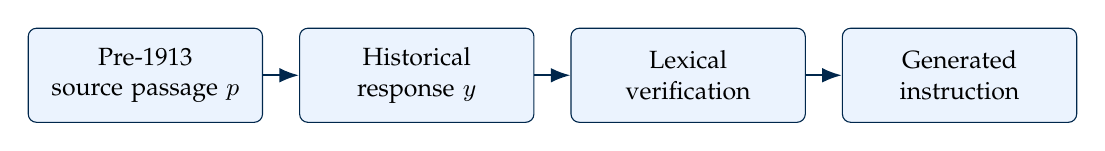
\begin{tikzpicture}[
                node distance=13pt,
                box/.style={draw=DarkBlue,rounded corners=3pt,fill=SoftBlue,
                    align=center,minimum height=34pt,text width=78pt,font=\small},
                arrow/.style={-{Latex[length=2.5mm]},thick,DarkBlue}
            ]
                \node[box] (source) {Pre-1913\\source passage $p$};
                \node[box,right=of source] (answer) {Historical\\response $y$};
                \node[box,right=of answer] (verify) {Lexical\\verification};
                \node[box,right=of verify] (question) {Generated\\instruction};
                \draw[arrow] (source) -- (answer);
                \draw[arrow] (answer) -- (verify);
                \draw[arrow] (verify) -- (question);
            \end{tikzpicture}}

            \vspace{5pt}
            \colorbox{SoftGray}{\parbox{0.94\linewidth}{\centering
                \textbf{Strict grounding:} $V(y) \subseteq V(p) \cup A$; every content word and numeral must be supported by the historical passage.}}
        \end{minipage}

        \vspace{7pt}
        \begin{minipage}{0.47\textwidth}
            \centering
            {\fontsize{17}{18}\selectfont\bfseries\textcolor{DarkBlue}{1,030}}\\[-1pt]
            \textbf{\histlima}\\
            \small Human-reviewed, including 30 multi-turn dialogues; 15 epochs.
        \end{minipage}
        \hfill
        \begin{minipage}{0.47\textwidth}
            \centering
            {\fontsize{17}{18}\selectfont\bfseries\textcolor{DarkBlue}{287,860}}\\[-1pt]
            \textbf{\histself}\\
            \small Responses stay fixed; only instructions are generated; 1 epoch.
        \end{minipage}
    }

    \headerbox{3. Evaluation I: Knowledge Cutoff Adherence}{name=evalcutoff,column=0,span=3,
        below=pretrain,above=bottom,borderColor=DarkBlue}{
        \begin{minipage}{\textwidth}
            \centering
            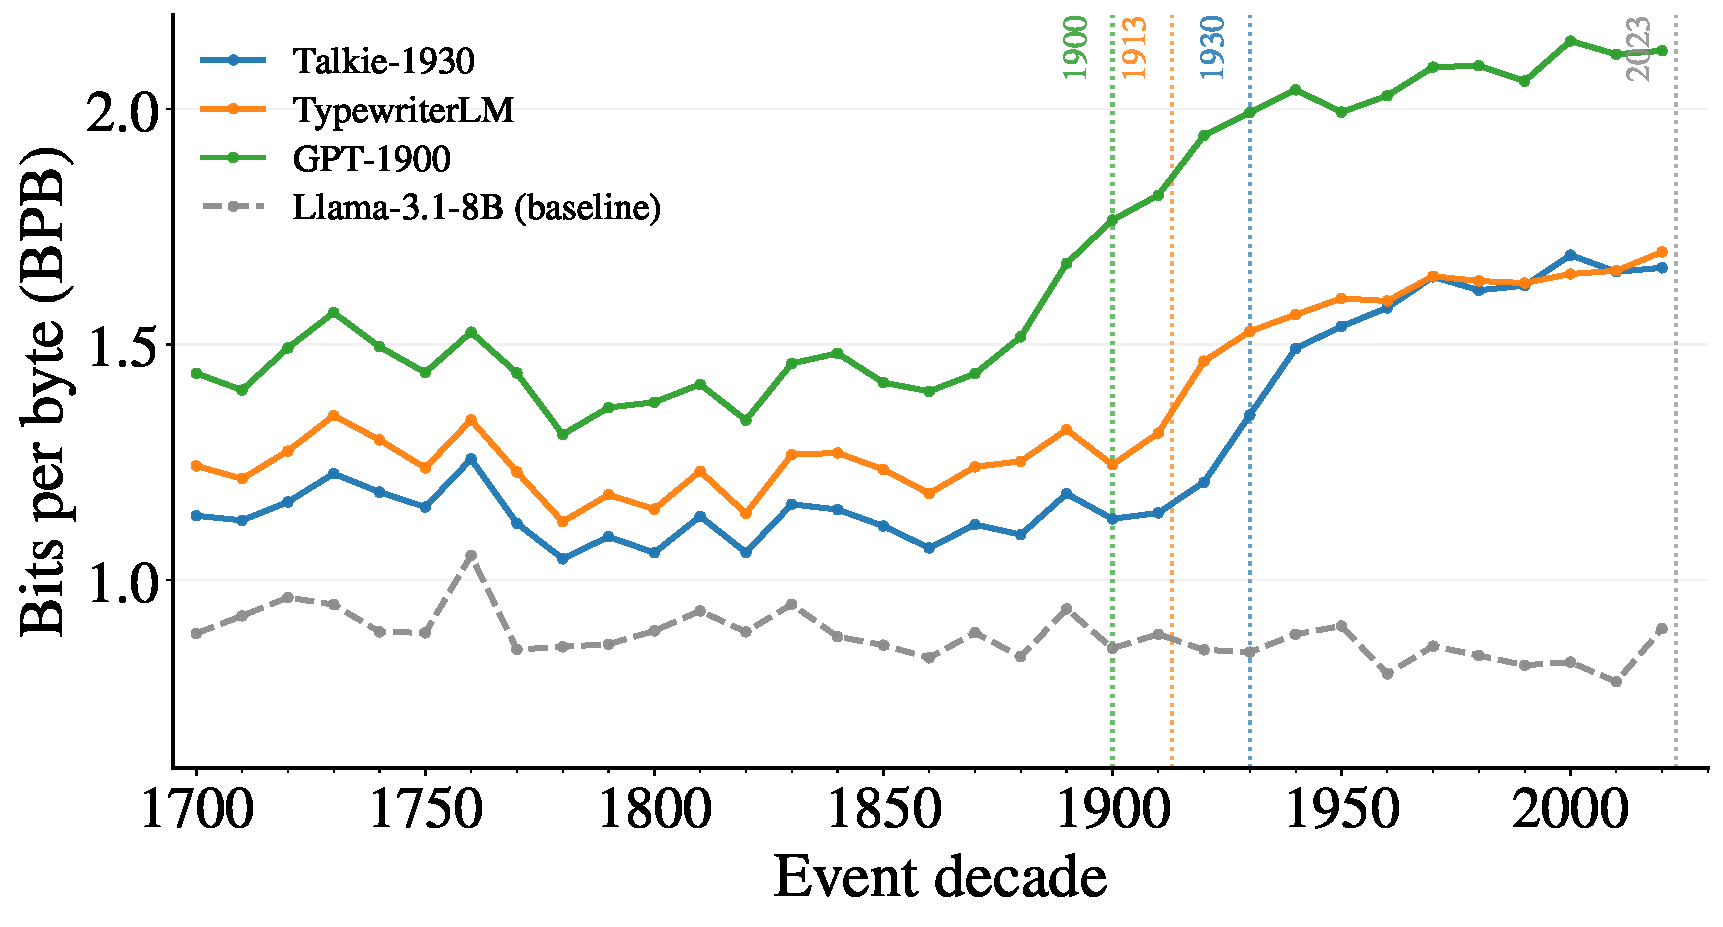
\includegraphics[width=0.94\linewidth]{perplexity_headline_by_decade.pdf}\\[-4pt]
            \small\textbf{Figure 2.} BPB surprisingness rises around History LM cutoffs.
        \end{minipage}

        \vspace{4pt}
        \begin{minipage}{0.46\textwidth}
            \centering
            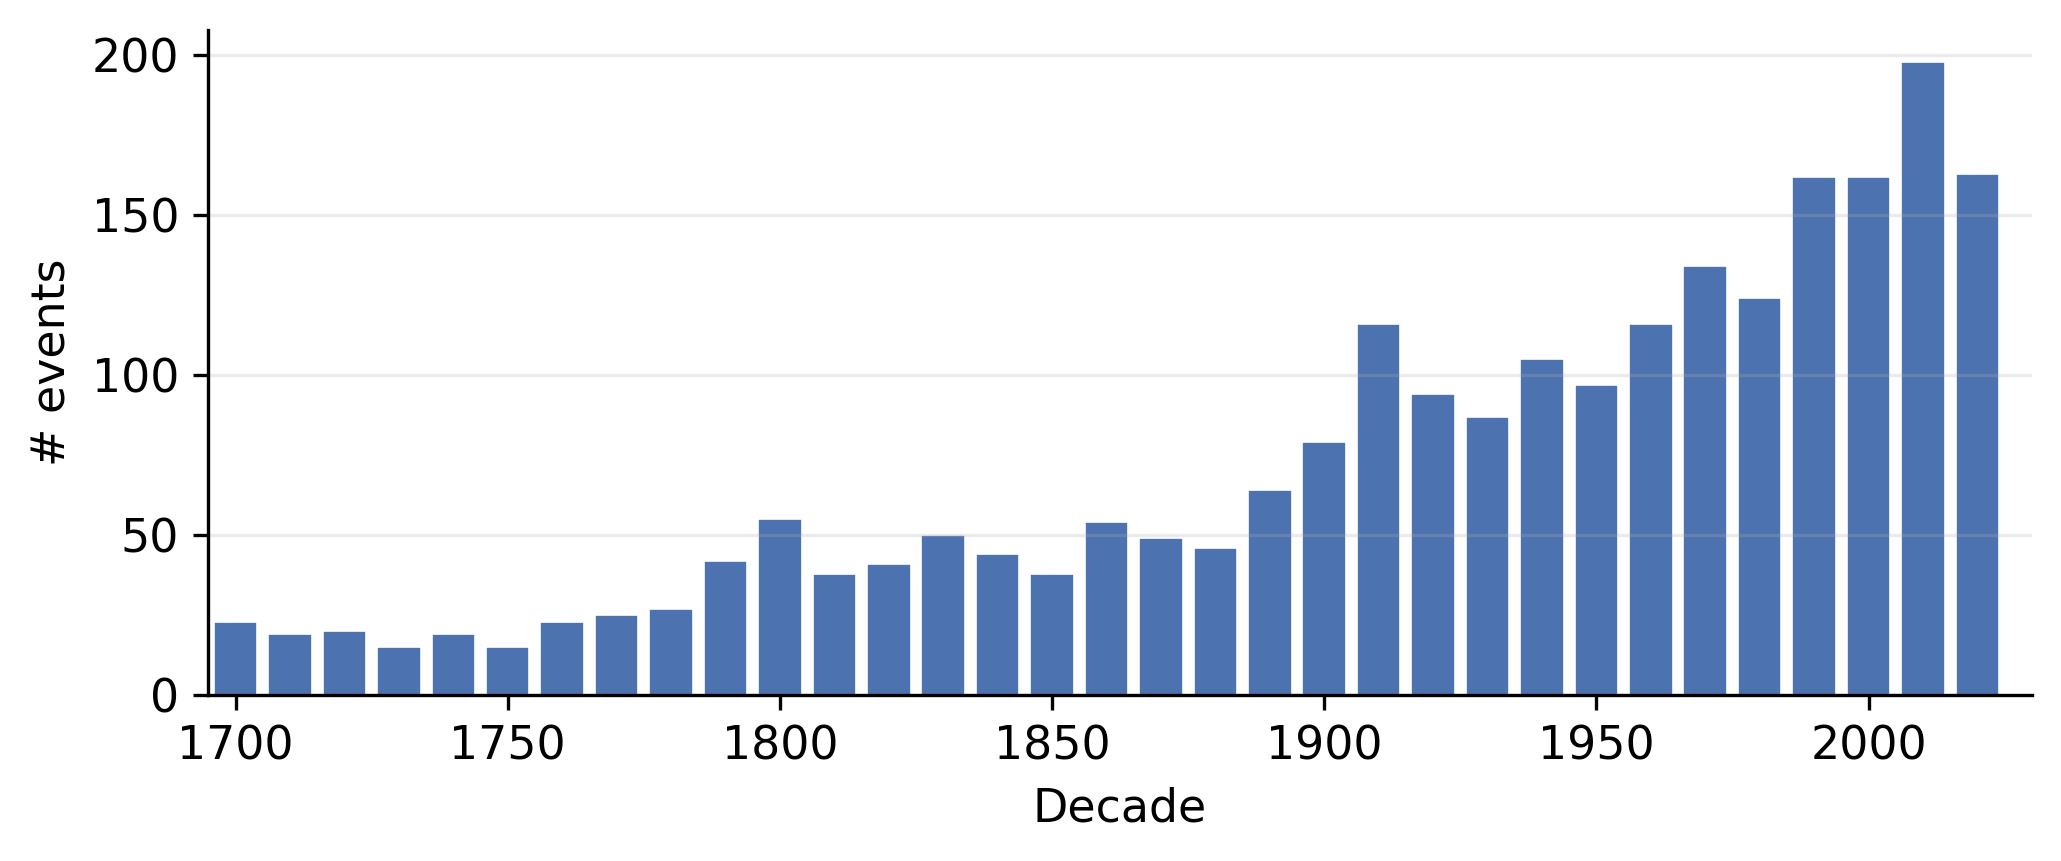
\includegraphics[width=\linewidth]{histevent_distribution.png}\\[-2pt]
            \small\textbf{History-Event:} 2,344 events spanning 1700--2025.
        \end{minipage}
        \hfill
        \begin{minipage}{0.50\textwidth}
            \small
            \textbf{Two complementary tests}
            \begin{enumerate}
                \item \textbf{Surprisingness:} bits per byte for event description and year.
                \item \textbf{Recall:} strict and relaxed factual recall before and after cutoff.
            \end{enumerate}
            \textcolor{DarkBlue}{\textbf{1,744 validated recall questions}} remain after filtering.
        \end{minipage}

        \vspace{6pt}
        \centering
        \resizebox{0.98\textwidth}{!}{%
            \begin{tabular}{llc cc cc cc}
                \toprule
                & & & \multicolumn{2}{c}{\textbf{Correctness (pre-cutoff)}$\uparrow$} &
                \multicolumn{2}{c}{\textbf{Leakage (post-cutoff)}$\downarrow$} & \multicolumn{2}{c}{\textbf{Count}} \\
                \cmidrule(lr){4-5}\cmidrule(lr){6-7}\cmidrule(lr){8-9}
                \textbf{Model} & \textbf{Size} & \textbf{Cutoff} & \textbf{Strict} & \textbf{Relaxed} & \textbf{Strict} & \textbf{Relaxed} & \textbf{pre} & \textbf{post} \\
                \midrule
                Talkie-1930 (base) & 13B & 1930 & 2.9 & 8.8 & 0.0 & 0.3 & 719 & 1025 \\
                Talkie-1930 (it) & 13B & 1930 & 34.5 & 53.3 & 0.0 & 0.9 & 719 & 1025 \\
                GPT-1900 (sft) & 3.29B & 1900 & 5.6 & 13.5 & 0.0 & 0.2 & 498 & 1246 \\
                Mr. Chatterbox & 340M & 1899 & 0.2 & 1.2 & 0.0 & 0.1 & 492 & 1252 \\
                TimeCapsuleLLM & 1.2B & 1875 & 0.0 & 0.5 & 0.0 & 0.0 & 394 & 1350 \\
                \midrule
                \rowcolor{SoftBlue}
                \twlm (base) & 7.24B & 1913 & 0.9 & 6.1 & 0.0 & 0.4 & 576 & 1168 \\
                \rowcolor{SoftBlue}
                \twlm (Self-Instruct) & 7.24B & 1913 & \textbf{6.2} & 20.3 & 0.1 & 0.6 & 576 & 1168 \\
                \rowcolor{SoftBlue}
                \twlm (LIMA) & 7.24B & 1913 & 3.6 & \textbf{20.5} & 0.0 & \textbf{0.3} & 576 & 1168 \\
                \bottomrule
            \end{tabular}}\par\vspace{1pt}
        \small\textbf{Table 2.} Full factual correctness and post-cutoff leakage results on \histevent.
    }

    \headerbox{4. Evaluation II: Benchmarks}{name=evalbench,column=3,span=3,
        below=posttrain,above=bottom,borderColor=DarkBlue}{
        \begin{minipage}[t]{\textwidth}
            \centering
            \textcolor{DarkBlue}{\textbf{General capability}}\\[3pt]
            \small
            \renewcommand{\arraystretch}{1.05}
            \setlength{\tabcolsep}{5pt}
            \resizebox{0.97\linewidth}{!}{\begin{tabular}{lccrrr}
                \toprule
                \textbf{Model} & \textbf{Era} & \textbf{Size} & \textbf{ARC-E} & \textbf{ARC-C} & \textbf{HellaSwag} \\
                \midrule
                Mr. Chatterbox & 1837--1899 & 0.34B & 33.9 & 22.9 & 28.2 \\
                TimeCapsule-v2 & 1800--1875 & 1.22B & 30.3 & 22.0 & 25.9 \\
                GPT-1900 & pre-1900 & 3.29B & 36.7 & 23.9 & 32.3 \\
                Talkie-1930 & pre-1930 & 13B & 55.8 & 35.6 & 49.8 \\
                GPT-2 XL & pre-2019 & 1.55B & 50.8 & 28.2 & 48.8 \\
                Qwen3-4B & pre-2025 & 4B & 77.4 & 51.6 & 65.9 \\
                \rowcolor{SoftBlue}
                \textbf{\twlm} & \textbf{1700--1913} & \textbf{7.24B} & \textbf{43.3} & \textbf{27.9} & \textbf{36.1} \\
                \bottomrule
            \end{tabular}}\par\vspace{1pt}
            \small\textbf{Table 3.} Accuracy (\%) on ARC-Easy, ARC-Challenge, and HellaSwag.

            \vspace{4pt}
            \colorbox{SoftGray}{\parbox{0.92\linewidth}{\centering\small
                \twlm outperforms smaller History LMs and reaches GPT-2 XL-level ARC-Challenge accuracy despite its 1913 cutoff.}}

            \vspace{10pt}
            \textcolor{DarkBlue}{\textbf{Temporal mismatch changes HellaSwag}}\\[3pt]
            \resizebox{0.86\linewidth}{!}{\begin{tabular}{lrrr}
                \toprule
                \textbf{Model} & \textbf{Original} & \textbf{Filtered} & \textbf{1800s prose} \\
                \midrule
                GPT-2 XL & 48.8 & 48.2 & \textcolor{PKUred}{41.2} \\
                Qwen3-4B & 65.9 & 66.2 & \textcolor{PKUred}{54.0} \\
                GPT-1900 & 32.3 & 32.3 & \textcolor{DeepGreen}{36.0} \\
                Talkie-1930 & 49.8 & 51.2 & \textcolor{DeepGreen}{52.3} \\
                \rowcolor{SoftBlue}
                \textbf{\twlm} & \textbf{36.1} & \textbf{36.2} & \textbf{40.0} \\
                \bottomrule
            \end{tabular}}\par\vspace{1pt}
            \small\textbf{Table 4.} Accuracy (\%) after topic filtering and historical-style rewriting.

            \vspace{4pt}
            \colorbox{SoftGray}{\parbox{0.92\linewidth}{\centering\small
                Rewriting into 1800s prose improves History LMs while reducing modern-model accuracy: language style is a major evaluation confound.}}
        \end{minipage}

        \vspace{10pt}
        \begin{minipage}[t]{\textwidth}
            \centering
            \textcolor{DarkBlue}{\textbf{Historically filtered AlpacaEval}}\\[3pt]
            \small
            \renewcommand{\arraystretch}{1.05}
            \resizebox{0.78\linewidth}{!}{\begin{tabular}{lrr}
                \toprule
                \textbf{Model vs. GPT-1900} & \textbf{Win} & \textbf{Loss} \\
                \midrule
                \twlm (LIMA) & 46.5 & 53.5 \\
                \twlm (Self-Instruct) & 42.0 & 58.0 \\
                \bottomrule
            \end{tabular}}\par\vspace{1pt}
            \small\textbf{Table 5.} Pairwise rates (\%) on 376 historically valid prompts.

            \vspace{4pt}
            \colorbox{SoftGray}{\parbox{0.88\linewidth}{\centering\small
                LIMA remains competitive with GPT-1900 even though every response is historically grounded.}}
        \end{minipage}

        \vspace{10pt}
        \begin{minipage}[t]{\textwidth}
            \centering
            \small
            \textcolor{DarkBlue}{\textbf{Historically filtered IFEval}}\\[3pt]
            \resizebox{0.92\linewidth}{!}{\begin{tabular}{lrrrr}
                \toprule
                \textbf{Model} & \textbf{P-S} & \textbf{P-L} & \textbf{I-S} & \textbf{I-L} \\
                \midrule
                GPT-1900 & 6.8 & 7.2 & 15.4 & 16.9 \\
                Talkie-1930-IT & 11.8 & 11.8 & 22.6 & 22.6 \\
                \rowcolor{SoftBlue}
                \twlm (LIMA) & 4.6 & 5.3 & 13.5 & 14.2 \\
                \rowcolor{SoftBlue}
                \twlm (Self-Instruct) & 10.3 & 10.3 & 18.1 & 19.1 \\
                \bottomrule
            \end{tabular}}\par\vspace{1pt}
            \small\textbf{Table 6.} Prompt/instruction accuracy under strict/loose matching.

            \vspace{4pt}
            \colorbox{SoftGray}{\parbox{0.88\linewidth}{\centering\small
                Self-Instruct broadly matches existing History LMs without unrestricted modern response generation.}}
        \end{minipage}

        \vspace{10pt}
        \centering
        \colorbox{SoftBlue}{\parbox{0.94\linewidth}{\centering\small
            \textbf{Overall:} historically aligned evaluation changes how capability should be interpreted.}}

    }

\end{poster}
\end{document}
